\chapter{Literature survey}

In my project plan I stated that "I will demonstrate my master level by understanding and simulating the dynamics of a 6 axis Robot arm."\cite{ProjectPlan}
This should be done by creating a model of the robot arm. 
To create the model of the robot arm, a literature review is necessary to lay out the best approach.\\
\medskip

\section{Field of study}

To start the literature review, a set of first keywords was needed. Through an expert interview with my company supervisor Trung Nguyen \cite{Trung} , who had already supervised other thesis projects in the domain of robotics, a list of keywords to start with was found in a quick discussion. Not all of these keywords were immediately clear, so it was necessary to find definitions for these. With the help of scientific databases and search engines, sources for these definitions could be found.\\




	\begin{itemize} [leftmargin=3cm]
		\item [\textbf{6 axis robot}] serial 6 degree of freedom robots (\cite{6axisRobot} with HANQuest)
		\item [\textbf{industrial robot arm}]  some form of jointed structure  achieved by the linking of a number of rotary and/or linear motions or joints( \cite{IndustrialRobotArm} with Science Direct)
		\item [\textbf{inverse kinematics}]  mathematical process of recovering the movements of an object with kinematic equations to determine the joint parameters that provide a desired position for each of the robot's end effectors (\cite{InvKinDef} with Wikipedia)
		\item[{\parbox[t]{0.25\linewidth}{\textbf{Peter Corke \\ robotics toolbox}}}] \parbox[t]{1\linewidth}{Matlab toolbox for the study and simulation of classical arm-type robotics, for example such things as kinematics, dynamics, and  trajectory generation (\cite{CorkeRoboticsToolbox} with Google search)}
		\item [\textbf{motion planning}]  find a sequence of valid configurations that moves the robot from the source to destination (\cite{MotionPlanning} with Google search)
		\item [\textbf{robot dynamics}] relationship between the forces acting on a robot mechanism and the accelerations they produce (\cite{RobotDynamics}, with Scholarpedia)
		\item [\textbf{ROS}] Robot Operating System - framework for writing robot software. It is a collection of tools, libraries, and conventions that aim to simplify the task of creating complex and robust robot behaviour across a wide variety of robotic platforms. (\cite{ROS} with Google search )
		%manual linebreak in item label
%		\item[{\parbox[t]{0.2\linewidth}{force here \\ a linebreak}}] Some text right of the label 
\end{itemize} 
\medskip

As seen in "Implementation of Robot Systems" \cite{IndustrialRobotArm}, the FANUC 210F is an articulated robot arm, also called a jointed arm. It is a 6 axis robot that has six rotational joints, each mounted on
the previous joint. This type of robot has the ability to reach a point within the working envelope in more than one configuration or position. 
As there are multiple configurations possible to reach the same position, path planning would become an important topic. 
This means through inverse kinematics  the motion of the joints needs to be determined without considering the local forces that cause them to move.
The robotics toolbox by Peter Corke was seen as a good tool for simulating these kinematics in MATLAB. 
When attaching the dynamics to this model, further simulations could be made to simulate the dynamic bahaviour of the robot arm and create a controller. %power demand to move the joints with the desired speed. 
%As it became clear, that it would be difficult to determine the inertias, spring and damping forces on the robot within the given time, a pure kinematic analysis was seen sufficient.
ROS, while being an advanced tool for robot control would not fall in the scope of this thesis, as it would rather be a tool for later in the process of integrating the robot into the production line.\\
\medskip

\section{In depth literature}

As stated in the online manual of MathWorks, "Kinematics is the study of motion without considering the cause of the motion, such as forces and torques." \cite{MathWorksInverseKinematics}
Inverse Kinematics, also called backward kinematics is the logical opposite to forward kinematics also called direct kinematics (See figure \ref{fig:FwVsInvKin}). 


\begin{figure}[H]
	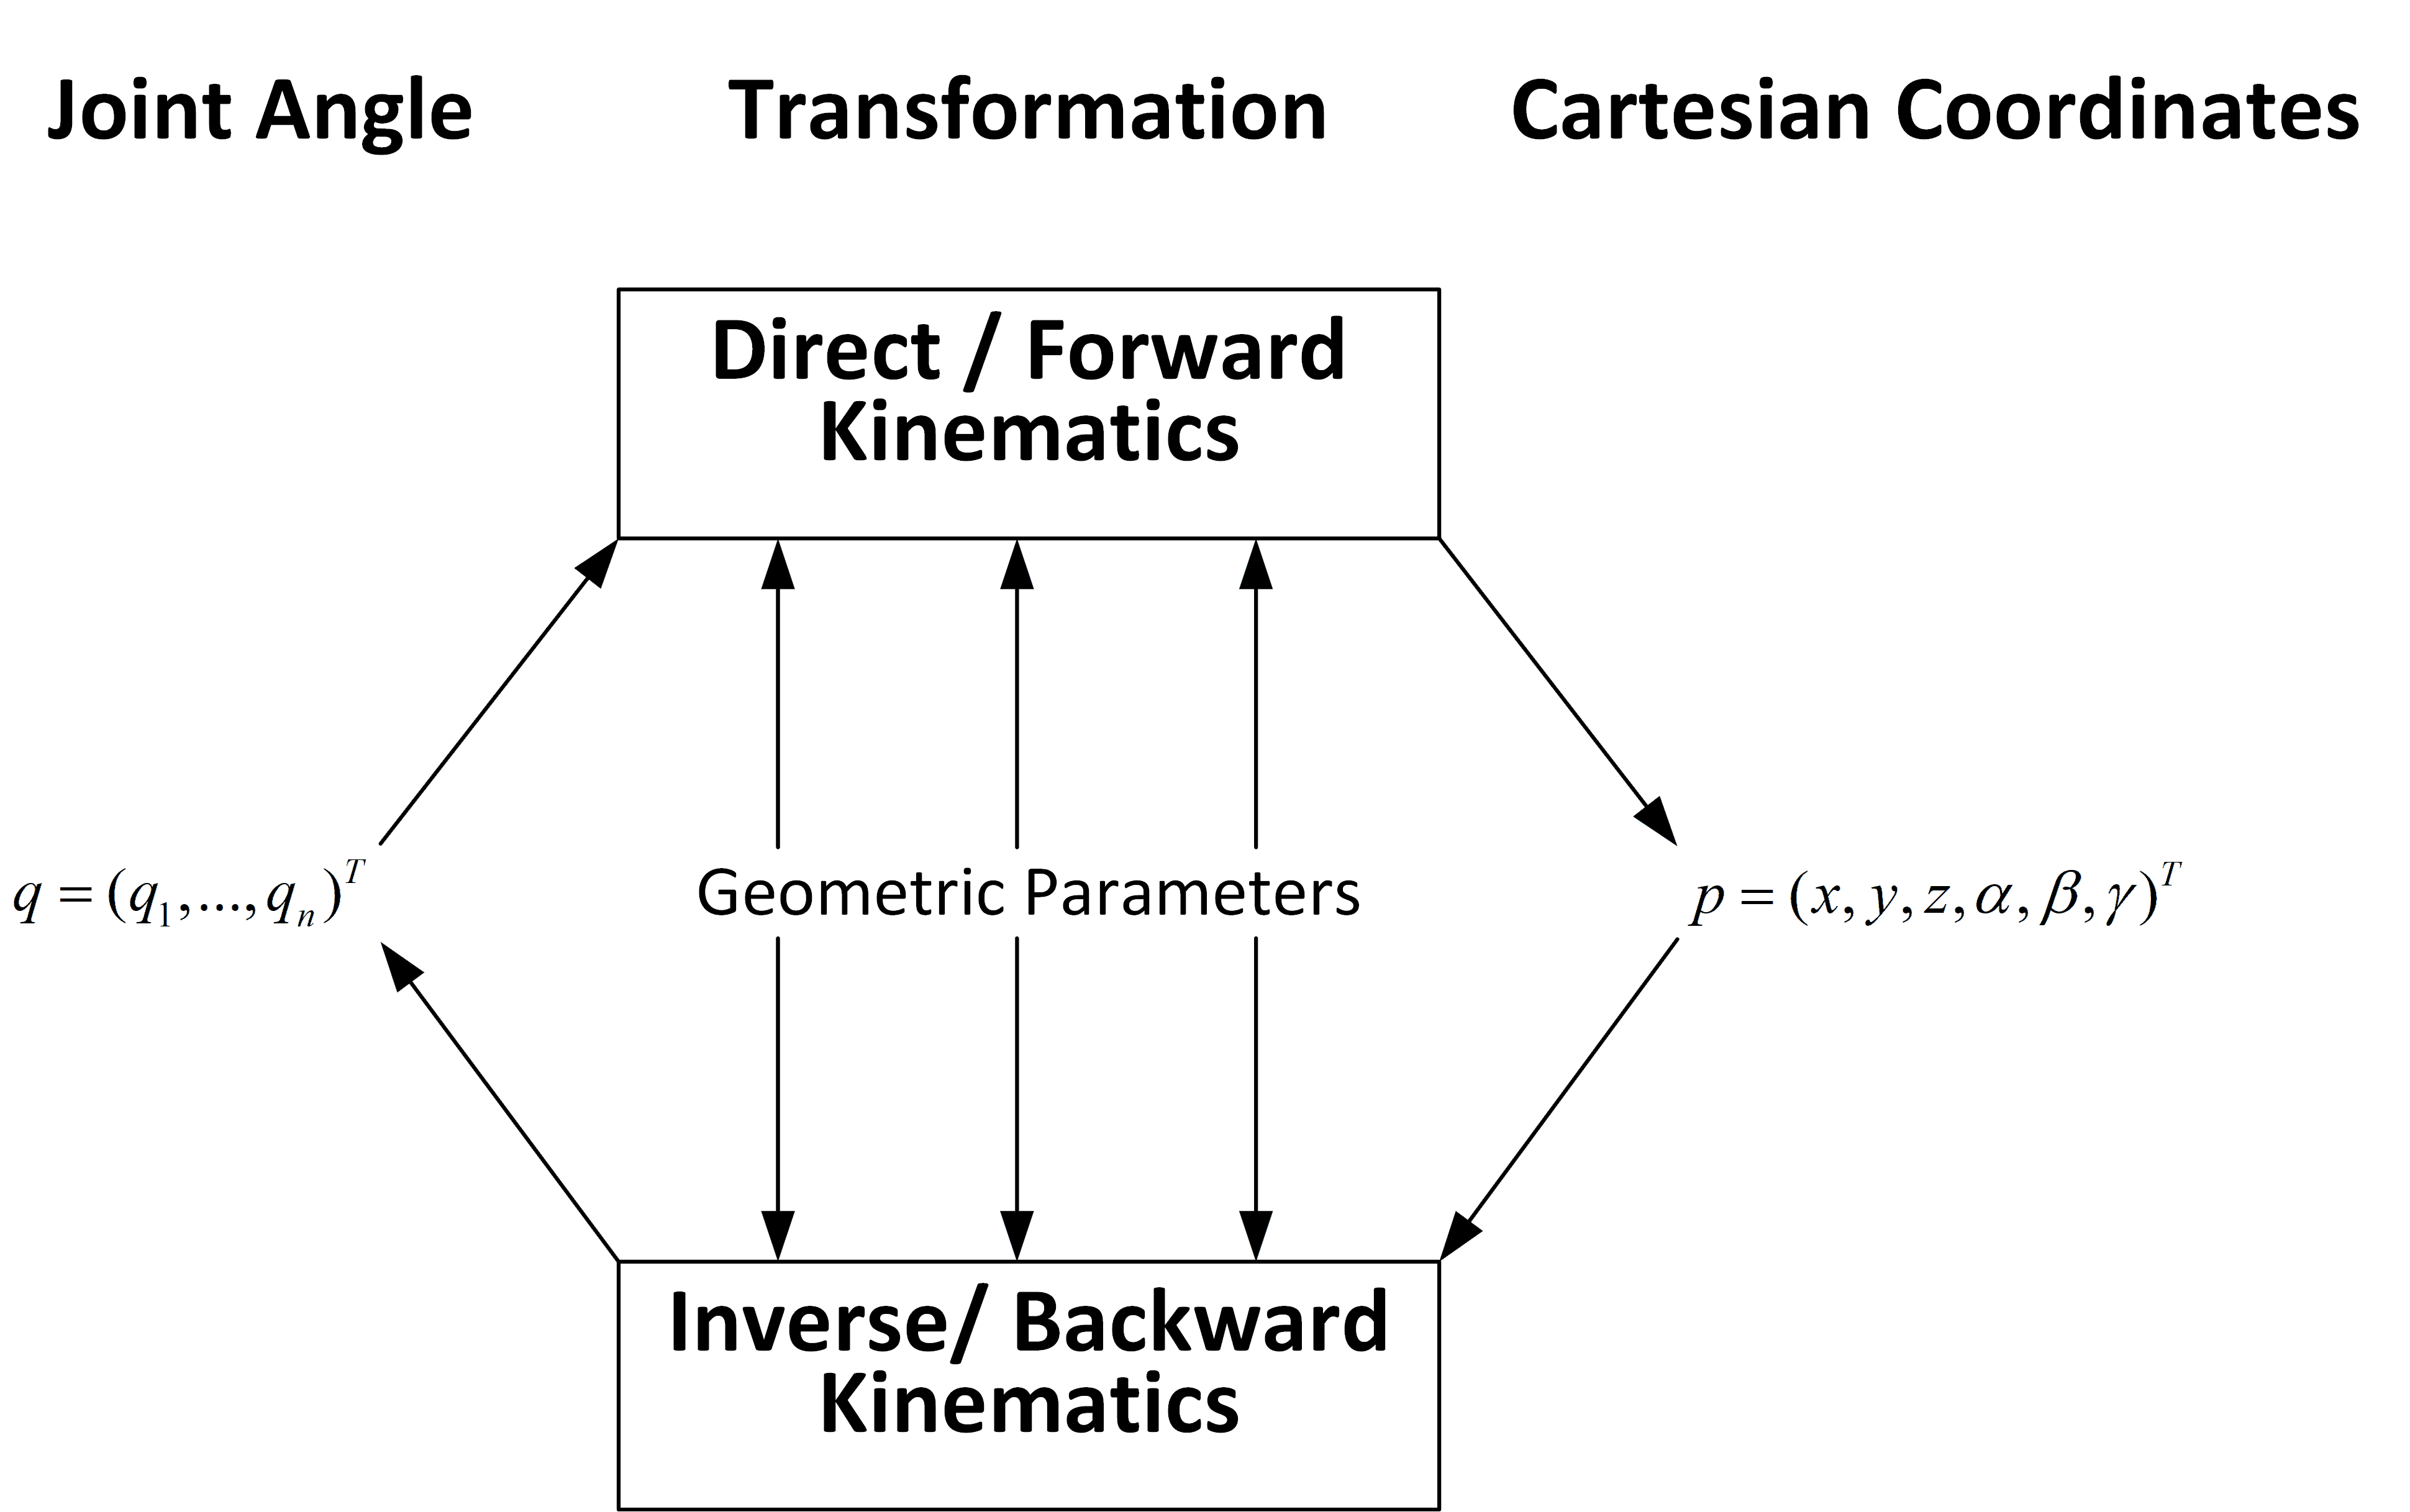
\includegraphics[
	width=0.95\linewidth,
	right,
	keepaspectratio,
	]{VisioDrawings/FWDvsINV_Kinematics_HighResTransp}
	\caption{Relation between inverse and forward kinematics translated from German Wikipedia site on inverse inematics \cite{forwardVsInverseKinematics}}
	\label{fig:FwVsInvKin}
\end{figure}

In the german wikipedia article on inverse kinematics \cite{inverseKinematikWiki}, the thesis "Verallgemeinerte inverse Kinematik für Anwendungen in der Robotersimulation und der virtuellen Realität" \cite{allgInvKin} is given as one of the main sources. 
This thesis work gives a good overview on the topic of inverse kinematics. 
As stated in this thesis work, the Denavit-Hartenberg notation is a robotic convention to map the local coordinate systems within a kinematic chain as found in robot arms.

As seen in "A Mathematical Introduction to Robotic Manipulation" \cite{MathIntroRobManip} (obtained through Semantic Scholar, search phrase: robotic convention), there are several other conventions besides the "Denavit-Hartenberg notation" used in the robotics research field like the the "product of exponentials formulation".
%Another overview on robotic conventions can be found in the Wikipedia article on robotic conventions \cite{RobConventionsWiki}. 
As most literature prefers a Denavit-Hartenberg fomulation of the kinematics (see \cite{MathIntroRobManip}), this convention will be chosen in this work as well.

Solutions for forward  kinematics are simple to obtain but solving inverse kinematics  has  been  one of  the  main  concerns  in  robot kinematics research. 
With more \ac{DOF}, solutions get more complex as non-linear equations with transcendental functions need to be solved. 
For this set of equations, no general algorithms are available.
Often algebraic, geometric and iterative methods for complex manipulators are used to find a solution to the inverse kinematic problem as stated by Tarun Pratap Singh et al. \cite{FwdInvAnalysRobManip}.

To find a suitable method for solving the inverse kinematic problem, a definition for the solution is needed:\\
\medskip
\\
\fbox{\parbox{\textwidth}{"A manipulator will be considered solvable if the joint variables can be determined by an algorithm that allows one to determine all sets of joint variables associated with a given position and orientation. [...] The algorithm should find all possible solutions" -Dr.-Ing. John Nassou\cite{invKinSeriallinkMani}}}
\bigskip

With this definition of solvability, all systems with revolute and prismatic joints with 6 \ac{DOF}  in a single series chain are solvable with the current available research. \cite{invKinSeriallinkMani}
As a quick search on HAN Quest with the search term "7 DOF inverse kinematics" suggests, there is currently onging research for the inverse kinematics problem in higher DOF manipulators with fuzzy logic as multiple articles following this approach can be found.\\
\\

As the goal is to find a suitable solution strategy for the inverse kinematic problem, it helps to map out the different types of methods.
Solution strategies can be split into two classes as stated by Dr.-Ing. John Nassou \cite{invKinSeriallinkMani}:\\
\medskip


%\parbox[t][3cm][t]{7cm}{\normalsize Closed-form solutions\\}
%\parbox[t][3cm][t]{7cm}{\normalsize Numerical solutions\\} 
%Text on two sides of the page:%https://tex.stackexchange.com/questions/107491/left-and-right-aligned-text-boxes
\fbox{\begin{minipage}[t]{0.6\textwidth}
	\textbf{{\large Closed-form solutions}}\\
	faster because analytical method\\
	will find all solutions\\
	Two approaches:\\
	\\
	\begin{minipage}[t]{0.4\textwidth}
		\textbf{{\large algebraic approach}}\\
	\end{minipage}
	\begin{minipage}[t]{0.4\textwidth}
	\begin{flushright}
	\textbf{{\large geometric approach}}\\
	\end{flushright}
\end{minipage}
\end{minipage}
\hfill
\begin{minipage}[t]{0.35\textwidth}
	\begin{flushright}
		\textbf{{\large Numerical solutions}}\\
		slower because of iterative nature\\
		not always find all solutions\\
	\end{flushright}
\end{minipage}}
\medskip

As numerical methods solve within an unknown number of operations, cannot always deliver  all solutions and depend on the users decision for accuracy, \cite{invKinSeriallinkMani} a closed-form solution will be preferred.

On HAN Quest, with the keywords "6DOF inverse kinematics" the article "Inverse Kinematics Solution and Optimization of 6DOF Handling Robot" \cite{invKinSolYanWu} can be found. This offers an  algebraic method to solve the inverse kinematic problem for 6 axis robots.
A similar approach is shown in "Forward and Inverse Kinematic Analysis of Robotic Manipulators" \cite{FwdInvAnalysRobManip}\\

As an alternative, a geometric modeling can be done as seen in "Workspace analysis and geometric modeling of 6 DOF Fanuc 200IC " \cite{geomModelingKamel}. 
A completely different approach is given in "A inverse kinematic solution of  a 6-DOF industrial robot using ANN" by using artificial neural networks \cite{invKinANNKSHITISH}.\\
%https://www.tu-chemnitz.de/informatik/KI/edu/robotik/ws2016/lecture-ik%201.pdf
%
%We will split all proposed manipulator solution strategies into two broad classes:Closed-form solutions and numerical solutions.Because of their iterative nature, numerical solutions generally are much slower than closed-form solutions and do not assure to really find all solutions.For most uses, we are not interested in the numerical approach to solve inverse kinematics.Here, we will restrict our attention to closed-form solutions.In this context, we search for solutions based on an analytic expression.
%Robots, for which a closed-form solution exists, are characterized either by having several intersecting joint axes or by having many twist angles αibe equal to0 or+/-90°.
%
With one of these methods, a solution can be found for the inverse kinematic problem.
This solution can then be verified with the robotics toolbox (Corke)

With this solution, a dynamic model of the robot can be created by attaching dynamics to the model as seen in "Control and Safety Mechanisms for a 3 DOF Manipulator with Human Interaction" \cite{KongWei} and "A mathematical introduction to Robotic Manipulation" \cite{MathIntroRobManip}. A complete example of a dynamic simulation of a 6 \ac{DOF} robot arm can be found in "Dynamic Multibody Simulation of a 6-DOF Robotic Arm" \cite{Dyn6DOFBinLi}

A controller for trajectory tracking can then be created with the model as seen in "Experimental Evaluation of Nonlinear Feedback and Feedforward Control Schemes for Manipulators" \cite{evalNonlinFeedForBackControl}

This controller could then be plugged into the real robot as stated in the "Control of a FANUC Robotic arm using MATLAB manual"  \cite{FANUCcontrolMatlab} An example of this can be found in "Modeling and analysis of a 6 DOF robotic arm manipulator" \cite{RobotModelAnalContrexampleJamshed}
























%In the module Systems modelling of the master course control systems at HAN, the 4+1 approach \ref{4+1} was presented. 
%
%\begin{figure}[H]
%	\centering
%	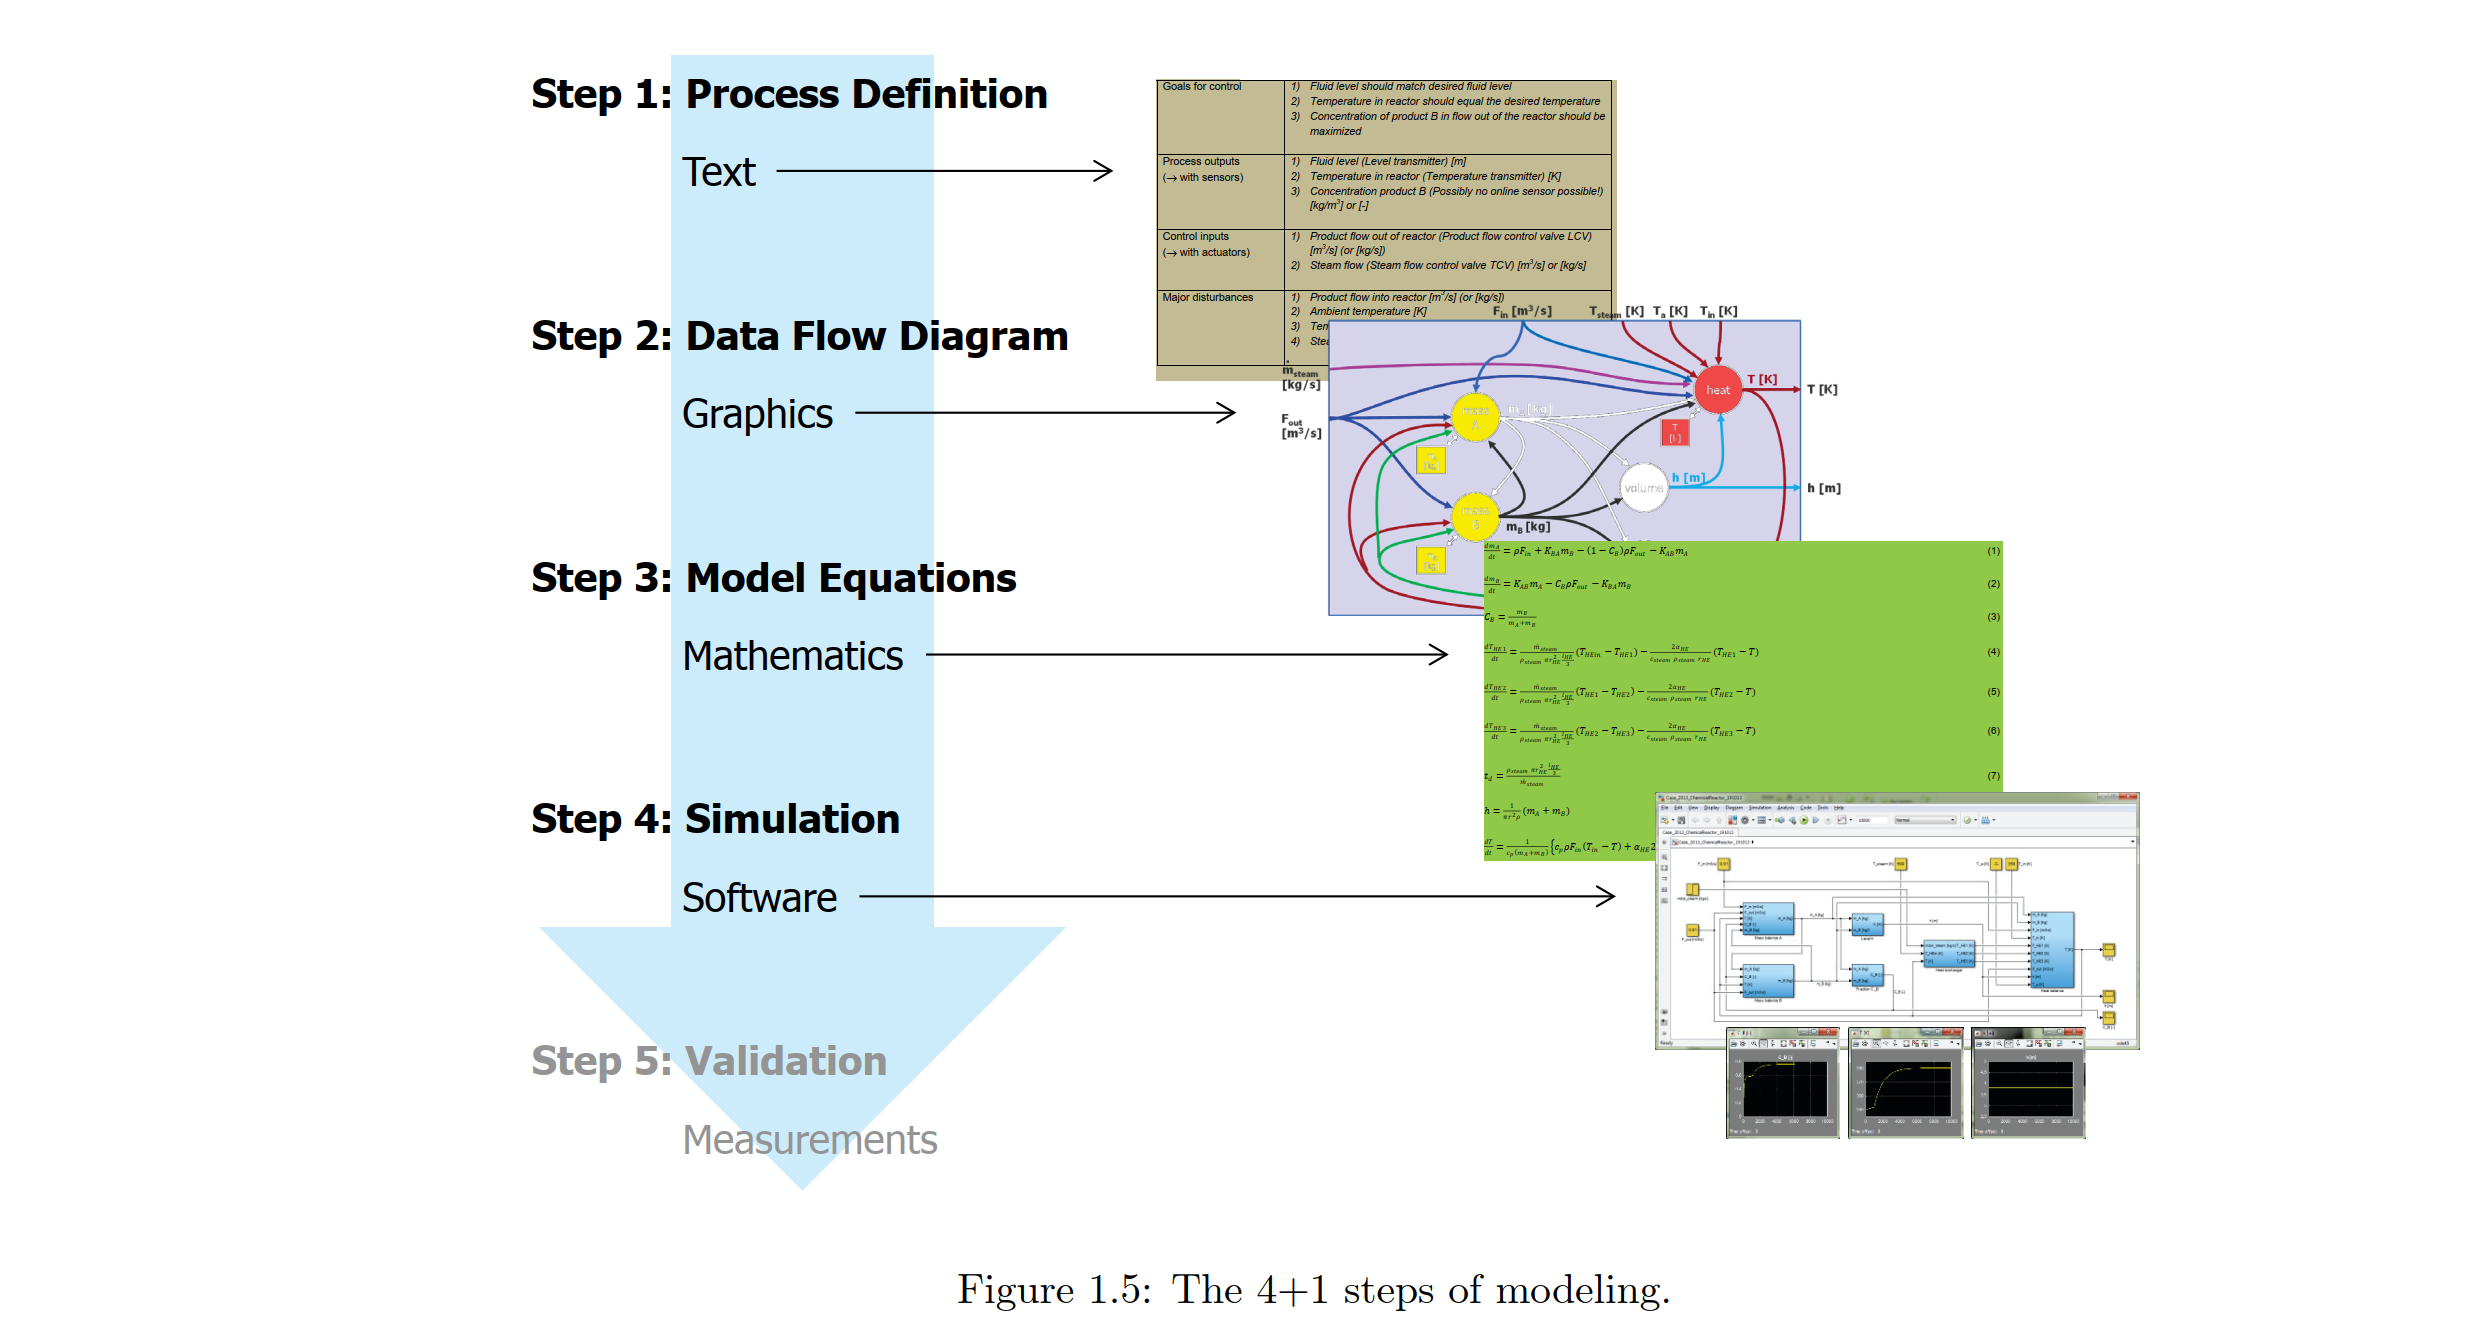
\includegraphics[
%	width=1\linewidth,
%	height=\paperheight,
%	keepaspectratio,
%	]{4+1Approach}
%	\caption{4+1 steps of modeling}
%	\label{fig:4+1}
%\end{figure}
%\pagestyle{empty}
%
%Starting from the process definition, model equations are derived with the help of a data flow diagram that lead to a simulation in software, e.g. Matlab. If possible, in the "+1" step, this model is validated with the real system.
%
%\section{Process Defintion}
%For object manipulation and other tasks, a robot arm needs to move to desired positions or track a given path. As the process focusses on the endpoint position of the robot arm, the process output can be defined as the xyz-position of the toolhead in space. The input, which can be used to control this output is the desired position. Another input that effects the output are objects attached to or carried by the robot arm. These can be considered disturbance inputs. From this, the process definition can be derived as seen in \ref{tab:ProcessDefinition}.
%
%\begin{table}[H]
%	\centering
%	\caption{Process Definiton}
%	\begin{tabular}{ll}
%		Goal for control:& Endpoint position of Robot arm   \\
%		Process output: & Endposition of Robot arm
%		 (sensor: measured with pulse encoders on the axes)   \\
%		Control inputs: & Electric power to the actuators
%		 (actuator: motor)  \\
%		Major disturbance & Carried object  
%	\end{tabular}
%\label{tab:ProcessDefinition}
%\end{table}